\documentclass{article}

\usepackage[utf8]{inputenc}
\usepackage[francais]{babel}
\usepackage[T1]{fontenc}
\usepackage{lmodern}
\usepackage{graphicx}
\usepackage{caption}
\usepackage{subcaption}
\usepackage{epstopdf}
\usepackage{array}
\usepackage{amsmath}
\usepackage{amssymb}
\usepackage{amsfonts}
\usepackage{amsopn}
\usepackage[usenames,dvipsnames]{color}
\usepackage[left=1.6cm,right=1.6cm,top=1.5cm,bottom=2cm]{geometry}

\usepackage{listings}
\definecolor{gray}{rgb}{0.4,0.4,0.4}
\definecolor{dkgreen}{rgb}{0.25,0.7,0.35}
\definecolor{dkred}{rgb}{0.7,0,0} 
\lstset{language=matlab,numbers=left,numberstyle=\tiny\color{gray},basicstyle=\rm\footnotesize,keywordstyle=\bfseries\color{dkred},frame=single,commentstyle=\color{gray}=small, stringstyle=\color{dkgreen}}

% Numbers and units
\usepackage[squaren, Gray]{SIunits}
\usepackage{sistyle}
\usepackage[autolanguage]{numprint}
%\usepackage{numprint}
\newcommand\si[2]{\numprint[#2]{#1}}
\newcommand\np[1]{\numprint{#1}}

% Matlab import
\usepackage{xparse}% for using parameters at the end block
\NewDocumentEnvironment{mylist}{m}{%
  \begin{#1}%
  % other code
}{%
  \end{#1}%
}

\NewDocumentEnvironment{mytable}{mm}
{\begin{table}[!ht]\centering}
{\caption{#2 Valeurs obtenues par le code du listing~\ref{lst:#1}.}\label{tab:#1}\end{table}}

\newcommand{\matlabplot}[2]
{\begin{figure}[!ht]\centering
\includegraphics[width=\textwidth]{img/#1.png}
\caption{#2 Graphique obtenu par le code du listing~\ref{lst:#1}.}\label{fig:#1}\end{figure}}


\newcommand{\matlabcode}[2]
{\lstinputlisting[caption={Contenu du fichier \lstinline{#1.m}
  contenant l'implémentation de la fonction \lstinline{#1}.
#2},label={lst:#1}]
{matlab/#1.m}
}

\DeclareMathOperator{\var}{Var}

\title{LFSAB1105 : Probabilités et statistiques \\ APP 2013 -- 2014}
\author{
\begin{tabular}{llll}
\textsc{Deschamps} & Samuel & \\
\textsc{Legat} & Benoît & 4896-11-00\\
\textsc{Peschke} & Lena & 5826-11-00\\
\textsc{Sanchez Falcon} & Alexandre & 2912-11-00\\
\textsc{Sedda} & Mélanie & 2246-11-00\\
\end{tabular}}
\date{\today}

\begin{document}

\maketitle
\pagenumbering{gobble}
\newpage


\textit{Tous les codes Matlab auquel nous ferons référence se trouvent dans l'annexe A du rapport.}
\pagenumbering{arabic}
\section{Question 1}
\subsection{Méthode des moments}
\subsection{Méthode graphique}
Soit l'échantillon aléatoire $X_1$,...,$X_n$ obtenu avec la loi de densité suivante (définie pour $x \geq 0$, avec $k$ et $c > 0$) :
$$ f(x) = \frac{k}{c}\left(\frac{x}{c}\right)^{k-1}\exp\left[-\left(\frac{x}{c}\right)^{k}\right] $$ 
On aimerait trouver un estimateur $\hat{\theta} = (\hat{k},\hat{c})$ pour $\theta = (k,c)$ en utilisant la régression linéaire.\\
Pour cela, notons que
$$ \ln(-\ln(1-F(x))) = k\ln(x)-k\ln(c) $$
Il suffit alors de choisir des points $x$ et d'estimer $F(x)$ grâce aux données empiriques $X_1$,...,$X_n$. La régression linéaire nous donnera des estimateurs $\hat{k}$ et $-\hat{k}\ln(\hat{c})$ dont nous pouvons facilement extraire $\hat{\theta}$. Pour simplifier les choses, on peut réindicer $X_1$,...,$X_n$ en $X_1'$,...,$X_n'$, de telle sorte que $X_1'<X_2'<$...$<X_n'$ (on suppose les $X_i$ obtenus différents). On évalue alors très simplement $F$ en chaque $X_i'$ : 
$$ \hat{F}(X_i') = i/n $$
On peut alors utiliser les $n-1$ premières valeurs de $X'$ pour effectuer la régression linéaire (le soucis avec la dernière c'est que $\hat{F}(X_n') = 1$ et donc $\ln(1-F)$ n'est pas défini). Par symétrie, il semble logique de rejeter aussi la première valeur (bien que la distribution Weibull ne soit pas symétrique). Voir code matlab pour l'implémentation.
\paragraph{}
Pour la suite, nous avons choisi $\theta = (2,2)$ comme paramètres à estimer et $n =1000$ comme taille d'échantillon.
Nous calculons $\hat{\theta}$ avec la régression linéaire, puis l'erreur quadratique totale $ERT$.\\
Voici les résultats obtenus pour un échantillon particulier (voir figure~\ref{fig:droite} pour la droite de régression linéaire) :
$$ \hat{\theta} = (1.9872,2.0368) $$
$$ ERT  = 0.0015 $$

\begin{figure}[!ht]
        \centering
        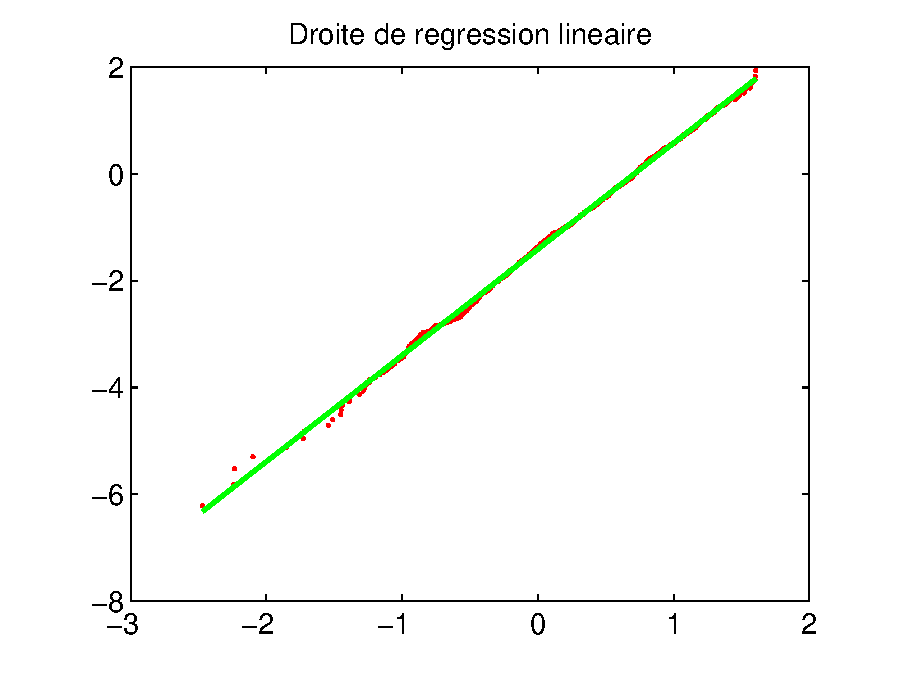
\includegraphics[width=0.5\textwidth]{graphes/droite_mg.eps}
        \caption{Droite de régression}\label{fig:droite}
\end{figure}

Pour étudier le biais et la variance de notre estimateur, nous avons reproduit notre estimation sur 500 échantillons. Voici les résultat pour la moyenne et la variance des séries $\hat{k}$, $\hat{c}$ et $ERT$. Les valeurs obtenues sont reprises dans la table~\ref{table:reg1}.

\begin{table}[!ht]
\centering
\begin{tabular}{|l|l|l|}
\hline
				& Moyenne 	& Variance\\
\hline
$\hat{k}$ 	& $1.9866$ 	& $0.0044$\\
$\hat{c}$ 	& $2.0020$ 	& $0.0012$\\
$ERT$		& $0.0057$	& $4.0814\cdot 10^{-5}$\\
\hline
\end{tabular}
\caption{Table des valeurs obtenues avec la méthode de régression linéaire pour 500 échantillons.}
\label{table:reg1}
\end{table}

Pour chaque série, nous avons produit un box-plot et un histogramme. Les graphes relatifs à $\hat{k}$ se retrouvent à la figure~\ref{fig:kmg}, ceux de $\hat{c}$ à la figure~\ref{fig:cmg} et ceux de $ERT$ à la figure~\ref{fig:ertmg}.

\begin{figure}[!ht]
        \centering
        \begin{subfigure}[b]{0.5\textwidth}
                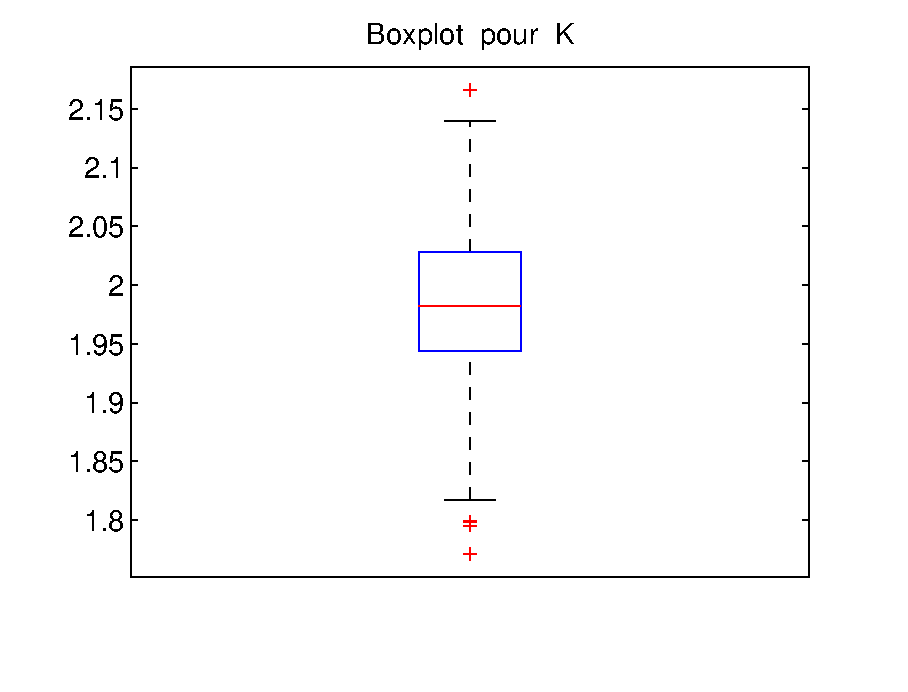
\includegraphics[width=\textwidth]{graphes/boxplot_kmg.eps}
        \end{subfigure}%
        ~
        \begin{subfigure}[b]{0.5\textwidth}
                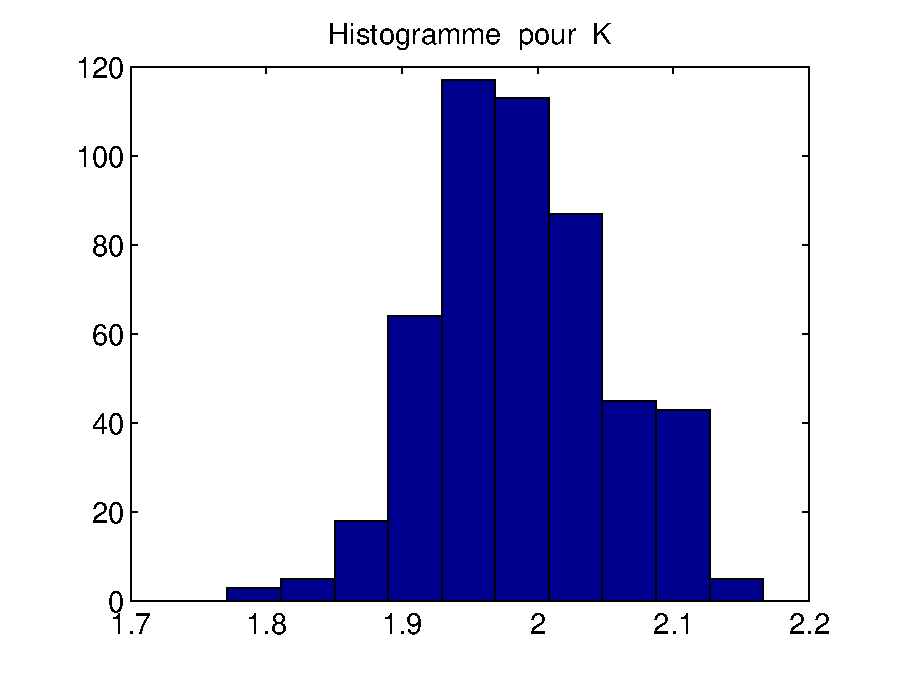
\includegraphics[width=\textwidth]{graphes/hist_kmg.eps}
        \end{subfigure}
        \caption{Graphes pour $\hat{k}$}\label{fig:kmg}
\end{figure}

\begin{figure}[!ht]
        \centering
        \begin{subfigure}[b]{0.5\textwidth}
                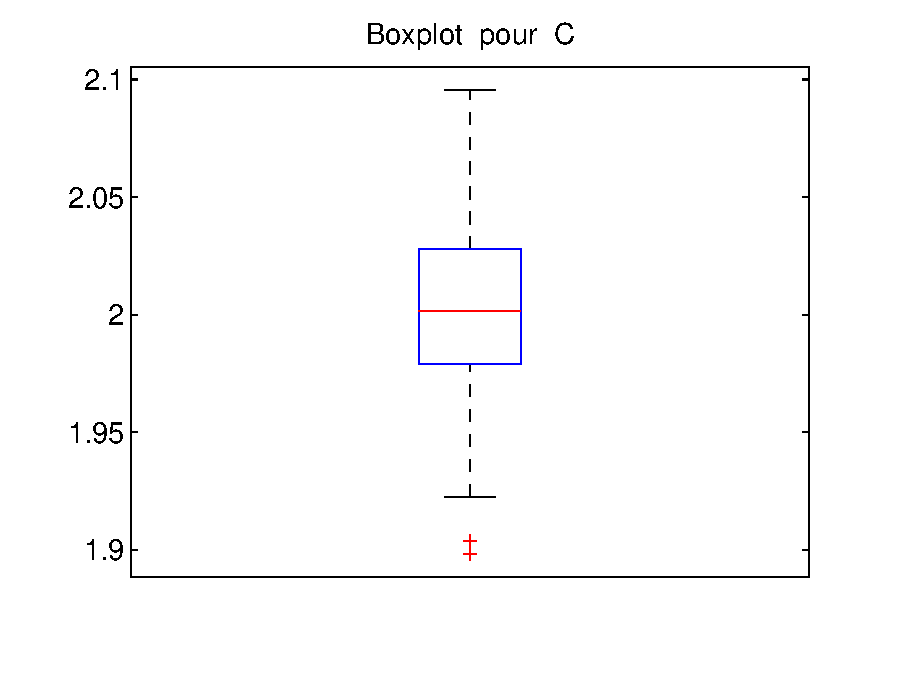
\includegraphics[width=\textwidth]{graphes/boxplot_cmg.eps}
        \end{subfigure}%
        ~
        \begin{subfigure}[b]{0.5\textwidth}
                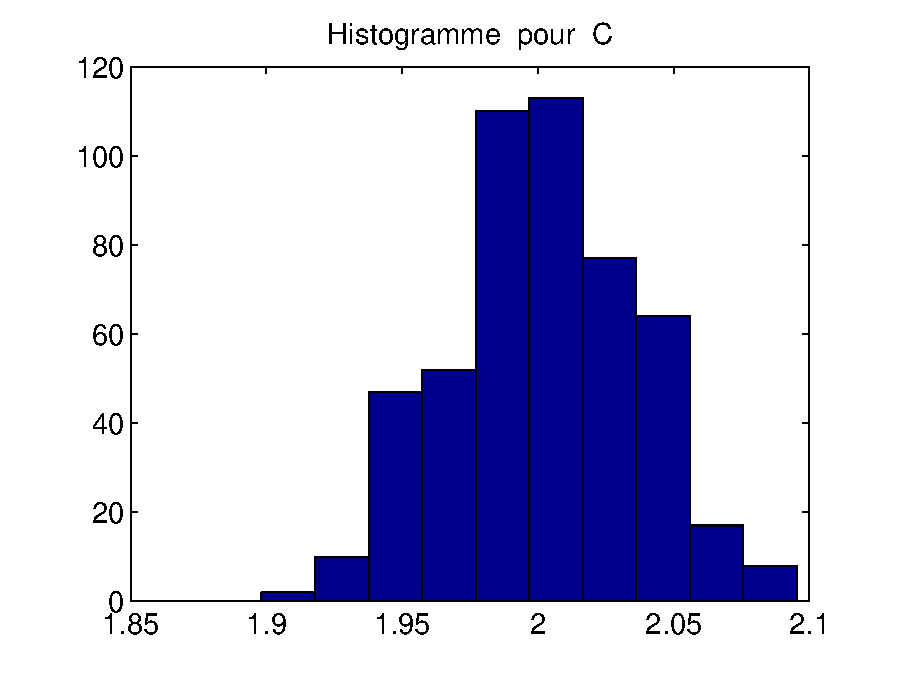
\includegraphics[width=\textwidth]{graphes/hist_cmg.eps}
        \end{subfigure}
        \caption{Graphes pour $\hat{c}$}\label{fig:cmg}
\end{figure}

\begin{figure}[!ht]
        \centering
        \begin{subfigure}[b]{0.5\textwidth}
                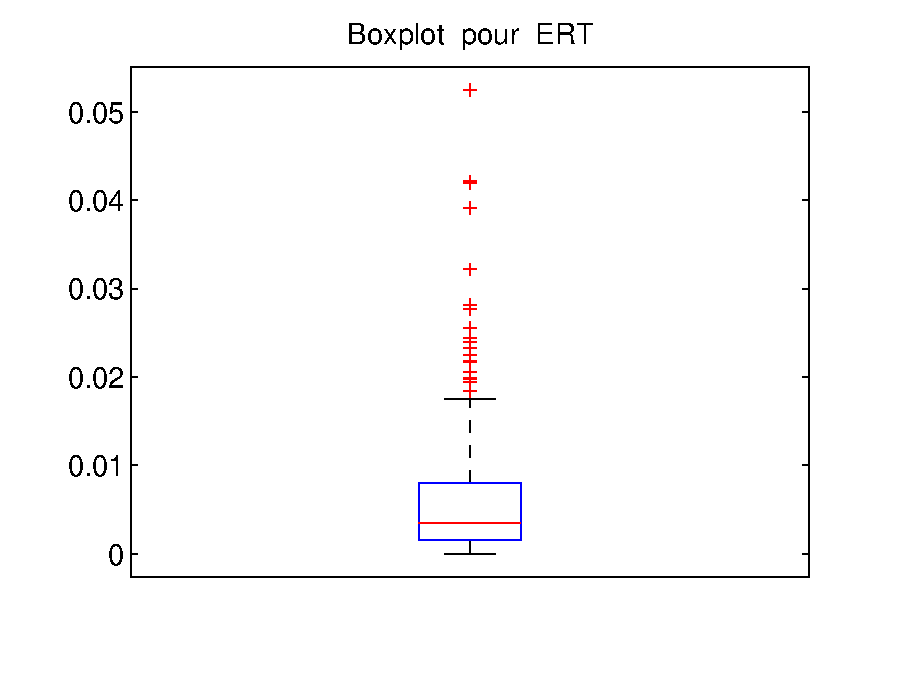
\includegraphics[width=\textwidth]{graphes/boxplot_ertmg.eps}
        \end{subfigure}%
        ~ 
        \begin{subfigure}[b]{0.5\textwidth}
                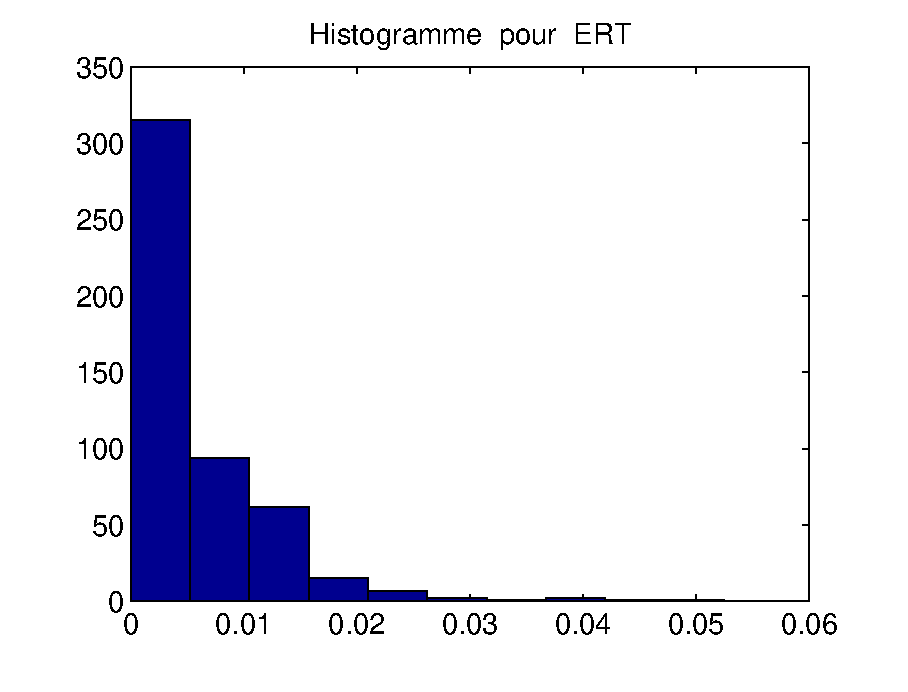
\includegraphics[width=\textwidth]{graphes/hist_ertmg.eps}
        \end{subfigure}
        \caption{Graphes pour $ERT$}\label{fig:ertmg}
\end{figure}

On ne peut pas dire avec certitude que notre estimateur est biaisé ou non. Si on devait estimer $\beta_0$ et $\beta_1$ tirés d'un modèle de type $Y = \beta_0 + \beta_1x + \epsilon$ avec $\epsilon$ venant d'une certaine distribution de moyenne nulle, alors la théorie prédit que les estimateurs fournis par la régression linéaire pour $\beta_0$ et $\beta_1$ sont non biaisés. Cependant, ici rien ne garantit la condition sur $\epsilon$, on va donc s'en tenir aux observations pour dire si nos estimateurs sont biaisés ou non.\\
Nous observons que notre estimateur pour $k$ est biaisé, tandis que celui pour $c$ ne l'est pas, du moins approximativement. Pour réduire le biais de $\hat{k}$ par rapport à $k$, on peut prendre des échantillons plus grands. On a aussi observé que rejeter plus de valeurs extrêmes réduisait le biais. Voici par exemples les résultat pour $n=10000$ en rejetant la première et dernière valeur (table~\ref{table:reg2}), et les résultats pour $n=1000$ en rejetant les 10 premières et les 10 dernières valeurs (table~\ref{table:reg10}).

\begin{table}[!ht]
\centering
\begin{tabular}{|l|l|l|}
\hline
				& Moyenne 	& Variance\\
\hline
$\hat{k}$ 	& $1.9960$ 	& $4.0303\cdot10^{-4}$\\
$\hat{c}$ 	& $1.9998$ 	& $1.1791\cdot10^{-4}$\\
$ERT$		& $5.3600\cdot10^{-4}$	& $3.5441\cdot 10^{-7}$\\
\hline
\end{tabular}
\caption{Régression linéaire, $n=10000$.}
\label{table:reg2}
\end{table}

\begin{table}[!ht]
\centering
\begin{tabular}{|l|l|l|}
\hline
				& Moyenne 	& Variance\\
\hline
$\hat{k}$ 	& $1.9924$ 	& $0.0035$\\
$\hat{c}$ 	& $1.9966$ 	& $0.0012$\\
$ERT$		& $0.0035$	& $2.2722\cdot 10^{-5}$\\
\hline
\end{tabular}
\caption{Régression linéaire, $n=1000$, valeurs extrêmes rejetées.}
\label{table:reg10}
\end{table}

Le résultat pour $n=10000$ montre que bien que $\hat{k}$ soit biaisé, il est asymptotiquement non biaisé. \\
Pour ce qui est de la distribution asymptotique de nos estimateurs, on peut voir dans les histogrammes (figures ~\ref{fig:kmg} et ~\ref{fig:cmg}) qu'elle est approximativement normale. \`A nouveau, si on avait pu affirmer se retrouver dans le cas d'un modèle de type $Y = \beta_0 + \beta_1x + \epsilon$, avec cette fois-ci $\epsilon$ distribué normalement et de moyenne nulle, alors la théorie prédit que les estimateurs pour $\beta_0$ et $\beta_1$ sont distribués normalement.\\
Enfin, on peut raisonnablement affirmer que nos estimateurs sont consistants, sachant que $\hat{c}$ est non biaisé, $\hat{k}$ est asymptotiquement non biaisé, et pour tous deux la variance tend vers $0$ lorsque $n$ tend vers l'infini.

\subsection{Méthode du maximum de vraisemblance}
\paragraph{Démonstration}
\noindent Partons de l'équation de maximum de vraisemblance : \\
\begin{equation}
\mbox{L}\left(\mbox{x}_{1},\cdots,\mbox{x}_{\mbox{n}}|\mbox{k },\alpha \right) = \left( \mbox{k} \alpha^{k} \right)^{n} \left( \prod\limits_{i=1}^{n} \mbox{x}^{\mbox{k}-1}_{i} \right) \mbox{exp}\left( -\alpha^{k} \sum\limits_{i=1}^n \mbox{x}^{k}_{i}\right)
\end{equation}
où $\alpha$ = $\dfrac{1}{c}$ . \\
Ensuite, nous travaillerons avec $\hat{\mbox{l}}$ = log$\left( \mbox{L} \right)$ tel que : 
\begin{equation}
\hat{\mbox{l}}(\mbox{x}_{1},\cdots,\mbox{x}_{\mbox{n}}|\mbox{k},\alpha) = \mbox{nlog}(\mbox{k}) + \mbox{nk log}(\alpha) + (\mbox{k}+1) \sum\limits_{i=1}^{n}\mbox{log}(\mbox{x}_{i}) - \alpha^{k} \sum\limits_{i=1}^{n} \mbox{x}^{k}_{i}
\end{equation}
avec $\hat{\mbox{l}}$ décomposé au maximum sous la forme d'une somme pour faciliter la dérivation. Par ailleurs, nous ne noterons plus les $\mbox{x}_{1},\cdots,\mbox{x}_{\mbox{n}}$ en argument par soucis de clarté. \\
Nous obtenons après dérivation en fonction de k et $\alpha$:
\begin{align}
\dfrac{\partial\hat{\mbox{l}}(\mbox{k},\alpha)}{\partial \alpha} &= \mbox{nk} \dfrac{1}{\alpha} - \sum\limits_{i=1}^{n} \mbox{x}^{k}_{i} \left( \mbox{k} \alpha^{\mbox{k}-1} \right) = 0 \label{eq:la} \\ \label{eq:lk}
\dfrac{\partial\hat{\mbox{l}}(\mbox{k},\alpha)}{\partial \mbox{k}} &= \dfrac{\mbox{n}}{\mbox{k}} + \mbox{n}\mbox{log}(\alpha) + \sum\limits_{i=1}^{n} \mbox{log}(\mbox{x}^{k}_{i}) - \sum\limits_{i=1}^{n} \dfrac{(\partial \alpha \mbox{x}_{i})^{\mbox{k}}}{\partial \mbox{k}} = 0.
\end{align}
Multiplions l'équation \ref{eq:la} par $\dfrac{\alpha}{\mbox{k}}$ :
\begin{equation}
\mbox{n} = \sum\limits_{i=1}^{n} \mbox{x }^{k}_{i} \alpha^{\mbox{k}} 
\end{equation}
il vient donc directement par la définition de $\alpha$ que :
\begin{equation}
\mbox{c} = \left(\sum\limits_{i=1}^{n} \mbox{x }^{k}_{i}\dfrac{1}{\mbox{n}}\right)^{\dfrac{1}{\mbox{k}}} \label{c}
\end{equation}
Développons à présent l'équation \ref{eq:lk}. \\ 
Nous utiliserons par ailleurs la propriété de dérivation suivante :
\begin{equation}
\dfrac{\partial \mbox{a}^{\mbox{x}}}{\partial \mbox{x}} = \mbox{log}(\mbox{a})~\mbox{a}^{\mbox{x}}
\end{equation}
après avoir développé la dernière dérivée partielle de l'équation \ref{eq:lk}, nous obtenons :
\begin{equation}
 \dfrac{\mbox{n}}{\mbox{k}} + \mbox{n}\mbox{log}(\alpha) + \sum\limits_{i=1}^{n} \mbox{log}(\mbox{x}^{k}_{i}) -  \sum\limits_{i=1}^{n}  \left[ \left[ \mbox{log}(\mbox{x}_{i}) + \mbox{log}(\alpha) \right] \alpha^{\mbox{k}} \mbox{x}^{k}_{i} \right] = 0. \label{8}
\end{equation}
Nous pouvons simplifier l'expression ci-dessus en utilisant le résultat obtenu en \ref{c} . Le terme de droite peut se réécrire :
\begin{equation}
\sum\limits_{i=1}^{n}  \left[ \left[ \mbox{log}(\mbox{x}_{i}) + \mbox{log}(\alpha) \right] \alpha^{\mbox{k}} \mbox{x}^{k}_{i} \right] = \mbox{n} \dfrac{\sum\limits_{i=1}^{n} \mbox{x}^{k}_{i} \mbox{~log}(\mbox{x}_{i})}{\sum\limits_{i=1}^{n} \mbox{x}^{k}_{i}} + \mbox{n}\mbox{log}(\alpha)
\end{equation}
en annulant les termes en log($\alpha$) dans \ref{8}, nous avons l'équation suivante :
\begin{equation}
\dfrac{\mbox{n}}{\mbox{k}} = \mbox{n} \dfrac{\sum\limits_{i=1}^{n} \mbox{x}^{k}_{i} \mbox{~log}(\mbox{x}_{i})}{\sum\limits_{i=1}^{n} \mbox{x}^{k}_{i}} - \sum\limits_{i=1}^{n} \mbox{~log}(\mbox{x}_{i})
\end{equation}
et nous obtenons le résultat souhaité :
\begin{equation}
\mbox{k} = \left[\dfrac{\sum\limits_{i=1}^{n} \mbox{x}^{k}_{i} \mbox{~log}(\mbox{x}_{i})}{\sum\limits_{i=1}^{n} \mbox{x}^{k}_{i}} - \dfrac{\sum\limits_{i=1}^{n} \mbox{~log}(\mbox{x}_{i})}{\mbox{n}}\right]^{-1}
\end{equation}

%b)
\paragraph{Echantillon, points candidats et fonction de vraisemblance}
La fonction \texttt{wblmle} nous permet de trouver un estimateur par la méthode du maximum de vraisemblance pour un échantillon aléatoire simple qui suit une loi de densité
$ f(x)= \frac{k}{c} \left(\frac{x}{c}\right)^{k-1} \exp \left[ -\left(\frac{x}{c}\right)^{k}\right] \mathbb{I}\{x \geq 0\}$ avec $k>0$ et $c>0$.
%b)
La première étape consiste à générer un échantillon $X_1,...,X_n$. Nous utilisons pour ce faire la fonction \texttt{wblrnd} avec un paramètre  $\theta$ au choix. Pour la suite de l'explication, posons $\theta = (k,c) = (3.7, 4.2)$. Nous construisons ensuite une grille de points candidats autour des valeurs de $k$ et $c$. La grille contient $101$ paires de point variant entre $(0.7k, 0.7c)$ et $(1.3k, 1.3c)$. Pour chaque paire de points, nous calculons le logarithme de la fonction de vraisemblance depuis la fonction \texttt{wblloglike}~:
$$LL(\theta=(k,c)) = \sum_{i=1}^{n}{\ln(f(x_i;\theta=(k,c)))} = n\ln(k) - kn\ln(c) + \sum_{i=1}^{n}{\left[(k-1)\ln(x_i) - \left(\frac{x_i}{c}\right)^{k}\right]}$$

\paragraph{Estimateurs et maximum de vraisemblance} Une fois les 101 points candidats évalués, nous cherchons le maximum parmi eux pour déterminer le $k$ et $c$ qui lui correspondent et qui deviennent $\hat{k}_{MLE}$ et $\hat{c}_{MLE}$, nos estimateurs de choix. C'est ce qui correspond à l'étape analytique $\frac{\partial LL(\theta)}{\partial \theta} = 0$.

%c)
\paragraph{Un exemple} En exécutant \texttt{wblmle(1000, 4.2, 3.7)} (où $n = 1000$ le nombre de $X_i$, $c = 4.2$, $k = 3.7$), nous obtenons, par exemple, $\hat{k}_{MLE} = 3.7000$ et $\hat{c}_{MLE} = 4.2504$.
L'erreur quadratique totale pour ces valeurs est $ERT_{MLE} = (\hat{k}_{MLE} - k)^2 + (\hat{c}_{MLE} - c)^2 = 0.0025$.

%d)
\paragraph{500 \'echantillons} La routine \texttt{MLE\_replicate} nous permet ensuite d'effectuer un certain nombre de réplications d'échantillons aléatoires simples et de calculer leurs $\hat{k}_{MLE}$, $\hat{c}_{MLE}$ et $ERT_{MLE}$ respectifs. Pour chacune des trois séries, nous calculons la moyenne et la variance. Les valeurs obtenues sont reprises dans la table~\ref{table:mle}.

\begin{table}[!ht]
\centering
\begin{tabular}{|l|l|l|}
\hline
				& Moyenne 	& Variance\\
\hline
$\hat{k}_{MLE}$ & 3.7006 	& 0.0086\\
$\hat{c}_{MLE}$ & 4.2003 	& 0.0014\\
$ERT_{MLE}$			& 0.0100	& 0.0001\\
\hline
\end{tabular}
\caption{Valeurs obtenues avec la méthode du maximum de vraisemblance pour 500 échantillons.}
\label{table:mle}
\end{table}

%e)
Pour chaque série, nous avons produit un box-plot et un histogramme. Les graphes relatifs à $\hat{k}_{MLE}$ se retrouvent à la figure~\ref{fig:kmle}, ceux de $\hat{c}_{MLE}$ à la figure~\ref{fig:cmle} et ceux de $ERT_{MLE}$ à la figure~\ref{fig:ertmle}.

\begin{figure}[!ht]
        \centering
        \begin{subfigure}[b]{0.4\textwidth}
                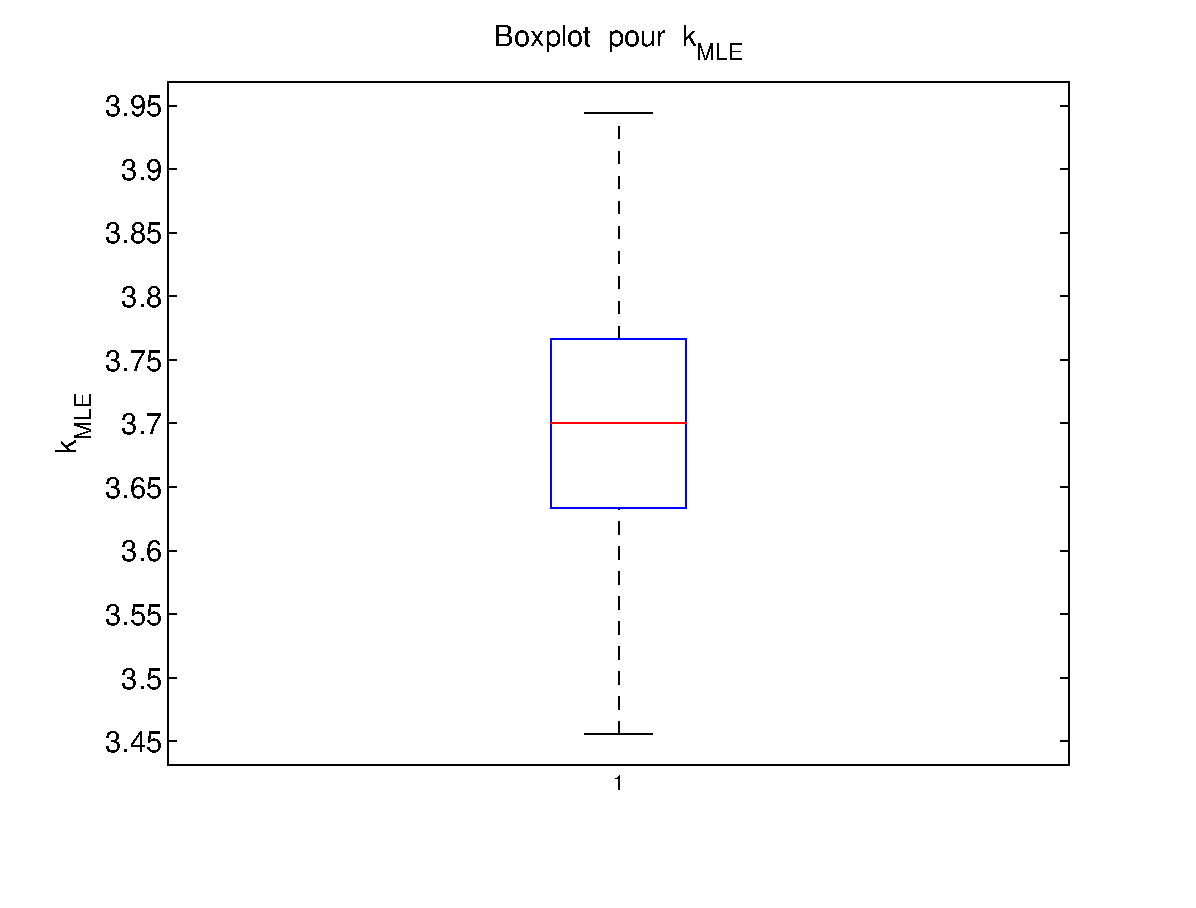
\includegraphics[width=\textwidth]{graphes/boxplot_kmle.eps}
        \end{subfigure}%
        ~
        \begin{subfigure}[b]{0.4\textwidth}
                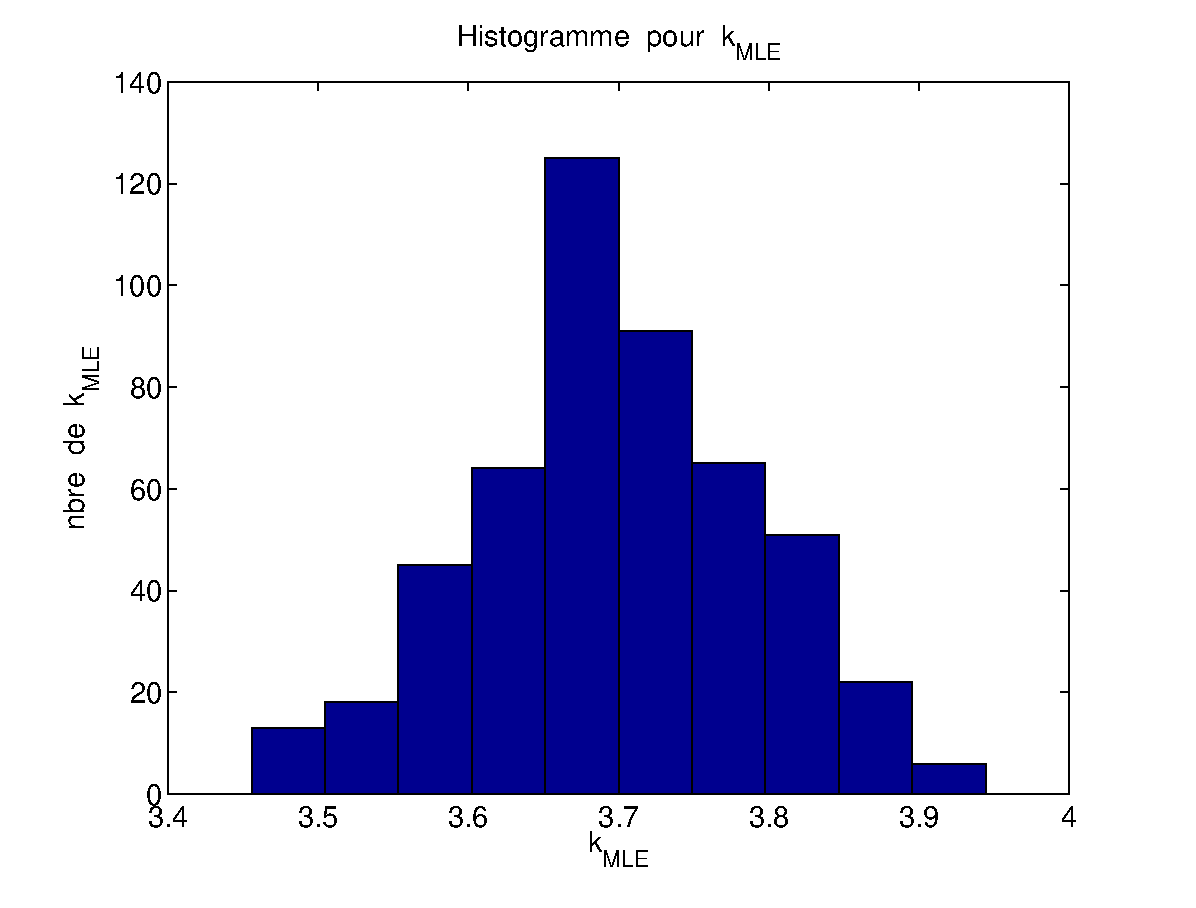
\includegraphics[width=\textwidth]{graphes/hist_kmle.eps}
        \end{subfigure}
        \caption{Graphes pour $\hat{k}_{MLE}$}\label{fig:kmle}
\end{figure}

\begin{figure}[!ht]
        \centering
        \begin{subfigure}[b]{0.4\textwidth}
                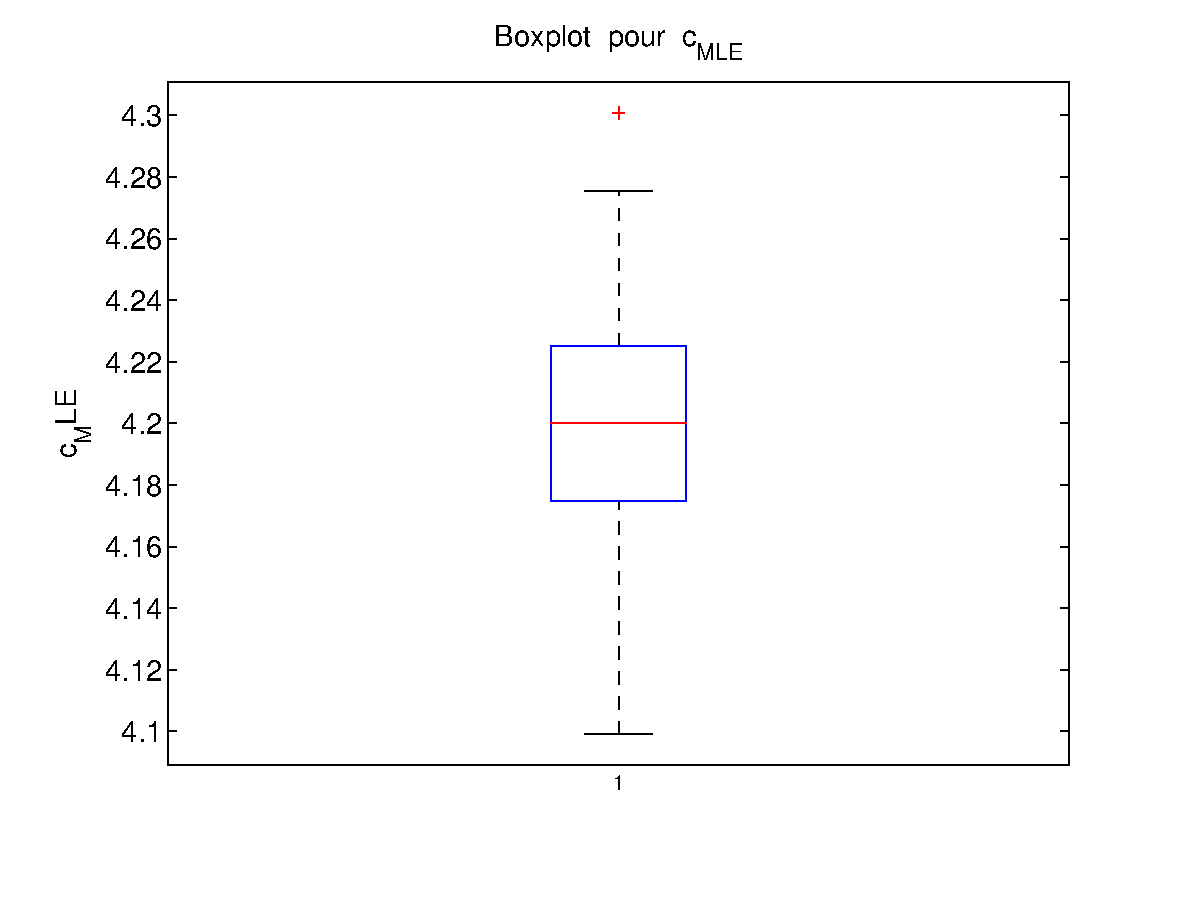
\includegraphics[width=\textwidth]{graphes/boxplot_cmle.eps}
        \end{subfigure}%
        ~
        \begin{subfigure}[b]{0.4\textwidth}
                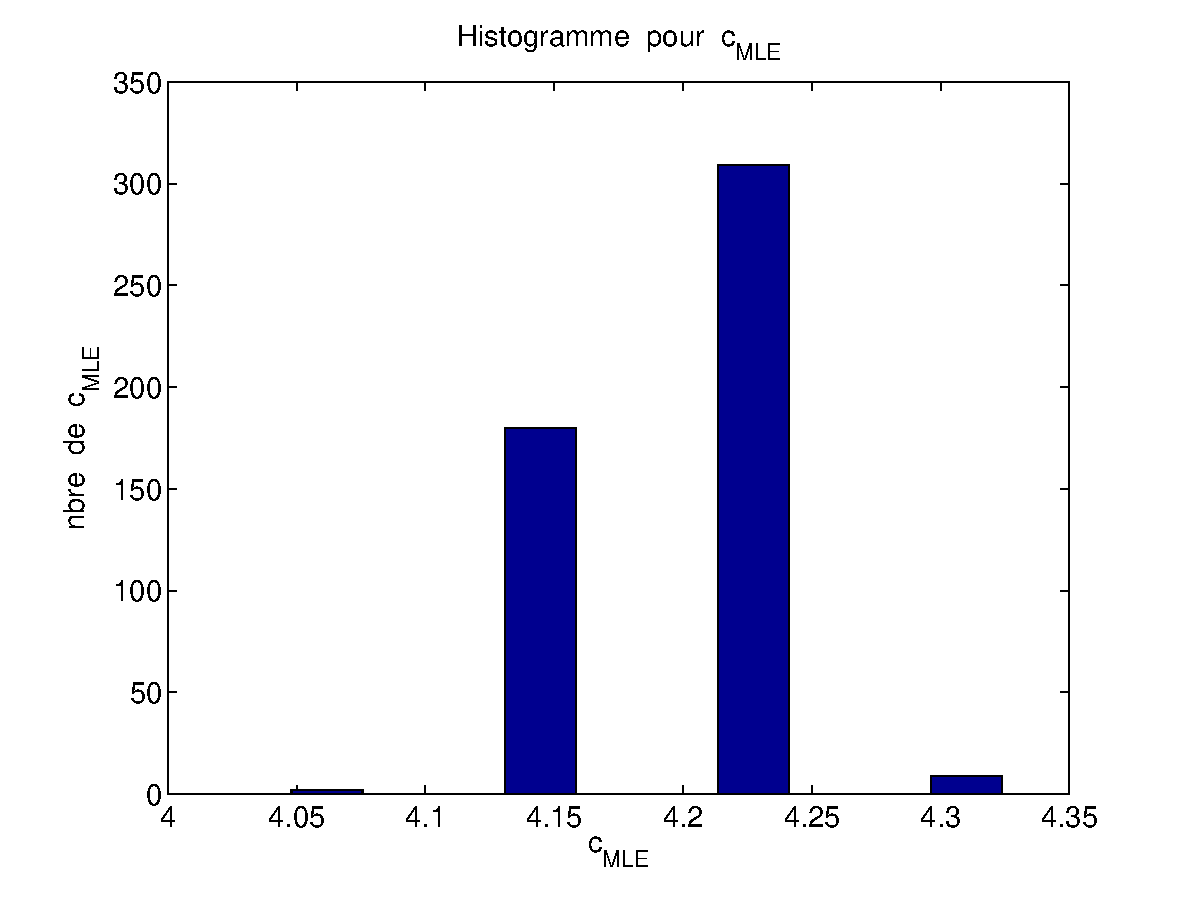
\includegraphics[width=\textwidth]{graphes/hist_cmle.eps}
        \end{subfigure}
        \caption{Graphes pour $\hat{c}_{MLE}$}\label{fig:cmle}
\end{figure}

\begin{figure}[!ht]
        \centering
        \begin{subfigure}[b]{0.4\textwidth}
                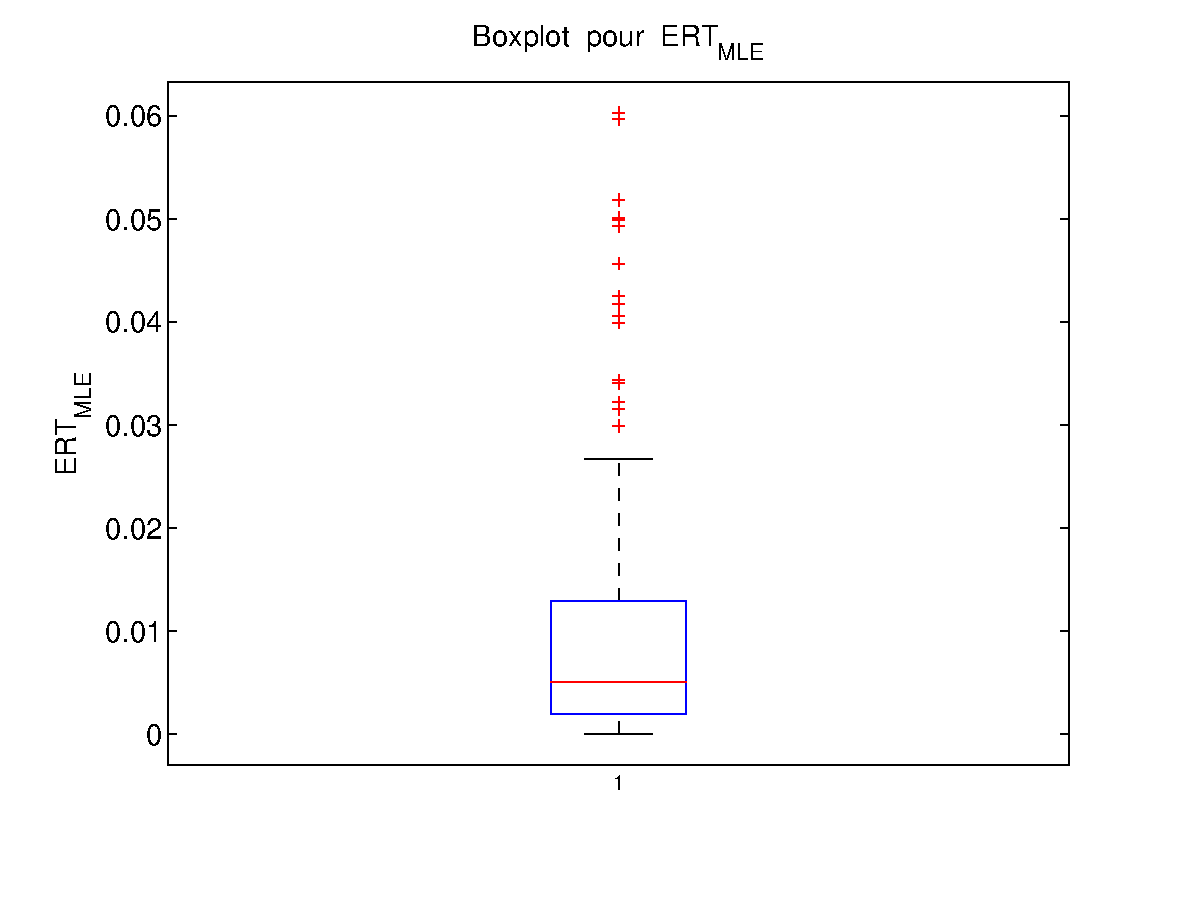
\includegraphics[width=\textwidth]{graphes/boxplot_ertmle.eps}
        \end{subfigure}%
        ~ 
        \begin{subfigure}[b]{0.4\textwidth}
                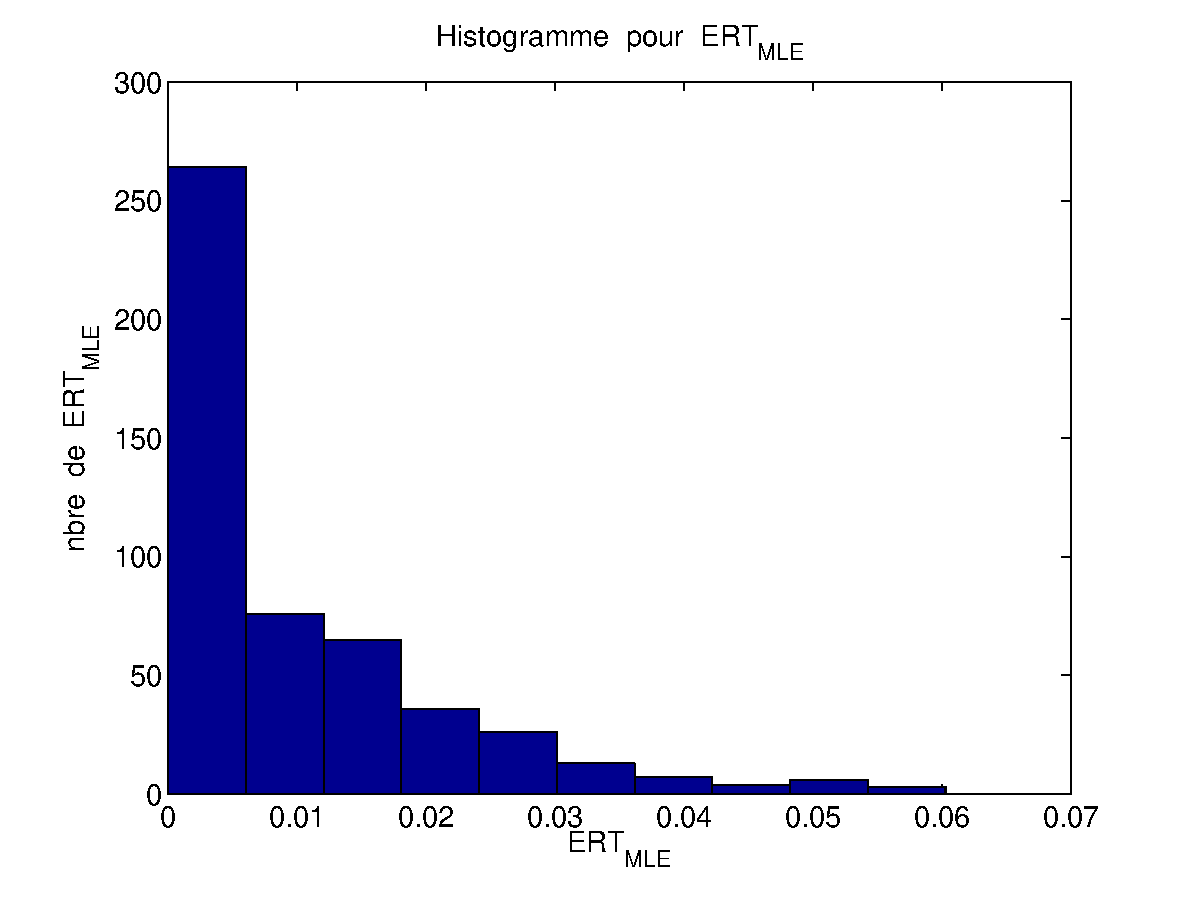
\includegraphics[width=\textwidth]{graphes/hist_ertmle.eps}
        \end{subfigure}
        \caption{Graphes pour $ERT_{MLE}$}\label{fig:ertmle}
\end{figure}

\paragraph{Biais, variance, consistence et distribution asymptotique}
La biais de notre estimateur $\hat{\theta}_{MLE}$ est négligeable; on peut donc raisonnablement dire qu'il est approximativement non-biaisé. En prenant des échantillons de plus en plus grand, on observe que la variance diminue. $\hat{\theta}_{MLE}$ est donc consistant. La table~\ref{table:MLE_n10000} reprend les valeurs obtenues pour $n = 10000$.
\begin{table}[!ht]
\centering
\begin{tabular}{|l|l|l|}
\hline
				& Moyenne 	& Variance\\
\hline
$\hat{k}_{MLE}$ & 3.7003 	& $8.5225 \cdot 10^{-4}$\\
$\hat{c}_{MLE}$ & 4.1997 	& $1.7429 \cdot 10^{-4}$\\
$ERT_{MLE}$		& 0.0010	& $1.7064 \cdot 10^{-6}$
\\
\hline
\end{tabular}
\caption{Maximum de vraisemblance, $n=10000$}
\label{table:MLE_n10000}
\end{table}
En ce qui concerne les distributions asymptotiques, les histogrammes montrent qu'elles sont approximativement normales. Notons toutefois que ces propriétés dépendent grandement des intervalles choisis initialement~: avec un intervalle plus grand autour des valeur réelles de $c$ et $k$, les résultats auraient été moins proches.



\subsection{Comparaison}

\section{Question 2}
\begin{enumerate}
  \item
    \begin{mytable}{val}{Table de différentes valeures des notes du test.}
      \begin{tabular}{ll}
        $n$                      & \np{252}\\
Moyenne                  & \np{1.059524e+01}\\
M\'ediane                & \np{1.050000e+01}\\
\'Ecart-type             & \np{2.642711e+00}\\
\'Etendue                & \np{1.250000e+01}\\
Coefficient de variation & \np{2.494244e-01}\\
Proportion de r\'eussite & \np{3.452381e-01}\\

      \end{tabular}
    \end{mytable}
  \item Utilisons la méthode des moments
    (qui donne la même chose que celle du maximum de vraissemblance pour
    une loi normale de toute façon).
    \begin{itemize}
      \item
        Pour la loi normale, on a
        \begin{align*}
          \bar{y} & = E(Y)\\
                  & = \mu\\
          \bar{y^2} & = E(Y^2)\\
                    & = \var(Y) + E(Y)^2\\
                    & = \sigma^2 + \mu^2
        \end{align*}
        ce qui donne
        \begin{align*}
          \mu & = \bar{y}\\
          \sigma^2 & = \bar{y^2} - \bar{y}^2.
        \end{align*}
      \item
        Pour la loi de Weibull, on a
        \begin{align*}
          \bar{y} & = E(Y)\\
                  & = \sqrt[m]{\alpha}\Gamma\left(1 + \frac{1}{m}\right)\\
          \bar{y^2} & = E(Y^2)\\
                    & = \var(Y) + E(Y)^2\\
                    & = \alpha^{2/m}\left(\Gamma\left(1 + \frac{2}{m}\right) -
                    \Gamma^2\left(1 + \frac{1}{m}\right)\right) + \alpha^{2/m}\Gamma^2\left(1 + \frac{1}{m}\right)\\
                    & = \alpha^{2/m}\Gamma\left(1 + \frac{2}{m}\right)
        \end{align*}
        ce qui donne
        \begin{align*}
          \mu & = \bar{y}\\
          \sigma^2 & = \bar{y^2} - \bar{y}^2.
        \end{align*}
    \end{itemize}
  \item
    La figure~\ref{fig:distrib} donne quelques exemple de distribution normale et de Weibull.
    On remarque que la distribution de Weibull a $f(x; \alpha, m) = 0$ $\forall x \leq 0$
    ce qui a du sens dans ce cas car une note ne peut pas être négative alors que
    la distribution normale a $f(x) > 0$ pour $f \leq 0$ même si la valeur est très faible
    si $\mu > 0$ et que $\sigma^2$ est suffisamment petit.

    \begin{figure}
      \centering
      \begin{subfigure}[b]{0.45\textwidth}
        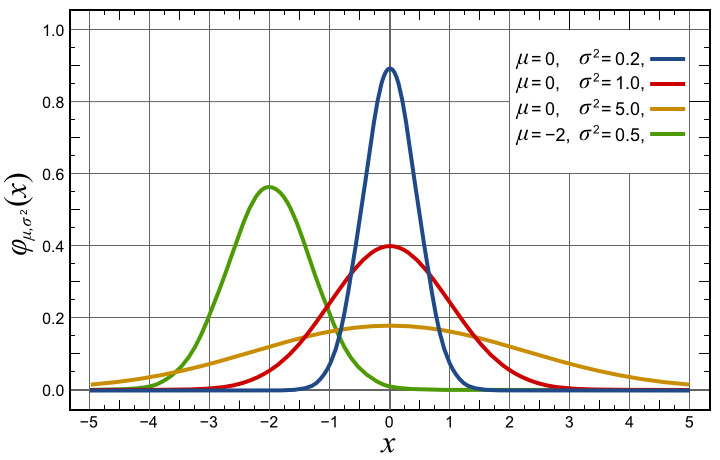
\includegraphics[width=\textwidth]{img/normal.png}
        \caption{Normal distribution}
        \label{fig:normal}
      \end{subfigure}%
      ~ %add desired spacing between images, e. g. ~, \quad, \qquad etc.
      %(or a blank line to force the subfigure onto a new line)
      \begin{subfigure}[b]{0.45\textwidth}
        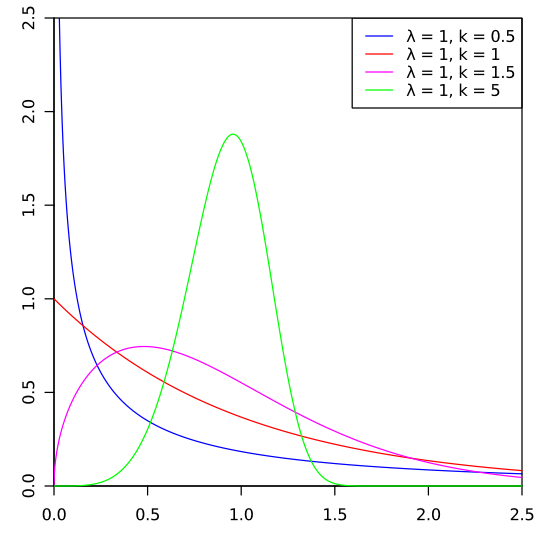
\includegraphics[width=\textwidth]{img/weibull}
        \caption{Weibull distribution}
        \label{fig:weibull}
      \end{subfigure}
      \caption{Comparison for Weibull and Normal distributions}
      \label{fig:distrib}
    \end{figure}
    De plus, la distribution normale est symétrique autour de $\mu$ alors que la distribution
    des notes d'un test n'est pas spécialement symétrique.
\end{enumerate}

\clearpage
\appendix

\section{Codes}
\matlabcode{val}{Cette fonction calculer différentes valeurs statistiques
des notes du test.}


\end{document}

